%
% Complete documentation on the extended LaTeX markup used for Insight
% documentation is available in ``Documenting Insight'', which is part
% of the standard documentation for Insight.  It may be found online
% at:
%
%     http://www.itk.org/

\documentclass{InsightArticle}

\usepackage[dvips]{graphicx}
\usepackage{subfigure}

%%%%%%%%%%%%%%%%%%%%%%%%%%%%%%%%%%%%%%%%%%%%%%%%%%%%%%%%%%%%%%%%%%
%
%  hyperref should be the last package to be loaded.
%
%%%%%%%%%%%%%%%%%%%%%%%%%%%%%%%%%%%%%%%%%%%%%%%%%%%%%%%%%%%%%%%%%%
\usepackage[dvips,
bookmarks,
bookmarksopen,
backref,
colorlinks,linkcolor={blue},citecolor={blue},urlcolor={blue},
]{hyperref}


%  This is a template for Papers to the Insight Journal. 
%  It is comparable to a technical report format.

% The title should be descriptive enough for people to be able to find
% the relevant document. 
\title{A Spline-Driven Image Slicer}

% 
% NOTE: This is the last number of the "handle" URL that 
% The Insight Journal assigns to your paper as part of the
% submission process. Please replace the number "1338" with
% the actual handle number that you get assigned.
%
\newcommand{\IJhandlerIDnumber}{xxxx}

% Increment the release number whenever significant changes are made.
% The author and/or editor can define 'significant' however they like.
\release{0.00}

% At minimum, give your name and an email address.  You can include a
% snail-mail address if you like.
\author{J\'er\^ome Velut}
\authoraddress{jerome.velut@gmail.com}

\begin{document}

%
% Add hyperlink to the web location and license of the paper.
% The argument of this command is the handler identifier given
% by the Insight Journal to this paper.
% 
\IJhandlefooter{\IJhandlerIDnumber}


\ifpdf
\else
   %
   % Commands for including Graphics when using latex
   % 
   \DeclareGraphicsExtensions{.eps,.jpg,.gif,.tiff,.bmp,.png}
   \DeclareGraphicsRule{.jpg}{eps}{.jpg.bb}{`convert #1 eps:-}
   \DeclareGraphicsRule{.gif}{eps}{.gif.bb}{`convert #1 eps:-}
   \DeclareGraphicsRule{.tiff}{eps}{.tiff.bb}{`convert #1 eps:-}
   \DeclareGraphicsRule{.bmp}{eps}{.bmp.bb}{`convert #1 eps:-}
   \DeclareGraphicsRule{.png}{eps}{.png.bb}{`convert #1 eps:-}
\fi


\maketitle


\ifhtml
\chapter*{Front Matter\label{front}}
\fi


% The abstract should be a paragraph or two long, and describe the
% scope of the document.
\begin{abstract}
\noindent
In this article, a spline driven image slicer algorithm is presented. It is
concretized through a vtkAlgorithm-inherited class that takes two inputs and
gives two outputs. The first input is the volume from which the slice should
reconstructed while the second one is the spline which tangent vector is used as
slicing plane normal. The first output is a 2D image resliced from the volume.
The second input gives the geometric information of the slice plane location in
the volume space. An example of use is given through a simulation of a dental
panoramic view from a MDCT volume. A straightened curved planar reformation is
also applied on vascular images.
\end{abstract}

\IJhandlenote{\IJhandlerIDnumber}

\tableofcontents
%
Slicing through volume data is a common task in scientific visualization. Lots
of existing image processing tools provide this necessary functionality as soon
as the visualization of 3D (or more) data has to be performed on a 2D screen.

In VTK, different ways are possible, depending on the particular slicing needed
by the end-user. The simplest is vtkExtractVOI if the desired slice is parallel
to the input image axes. This method is used in ParaView in the Slice 
Representation. The most sophisticated is the vtkImageReslice filter in which
the cutting plane may be oriented arbitraly in the volume space. Though these
filter are able to resample from 3D to 3D, this work focus on 2D slicing from
3D images.

The algorithm presented here aims at computing the slicing orientation of a
vtkImageReslice filter directly from an input spline curve. This orientation
is defined as the Frenet-Serret frame at each point of the spline. In the 
following, a Frenet-Serret variant is proposed in order for the spline tangents
to be used as slice plane normals. An application on mandibule panoramic 
visualisation is presented, as well as an implementation of the Straightened
Curved Planar Reformation in vascular imaging.
%
\section{Frenet-Serret frame along a curve}
\cite{FRE52, SER51}
%
\subsection{Initial definition}
%
\subsection{Coherent consecutive normals computation}
%
\section{Image slicing}
%
\subsection{Inputs}
%
\subsection{Outputs}
%
\subsection{Parameters}
%
\section{Applications}
%
\subsection{Dental panoramic visualisation}
\begin{figure}
\centering
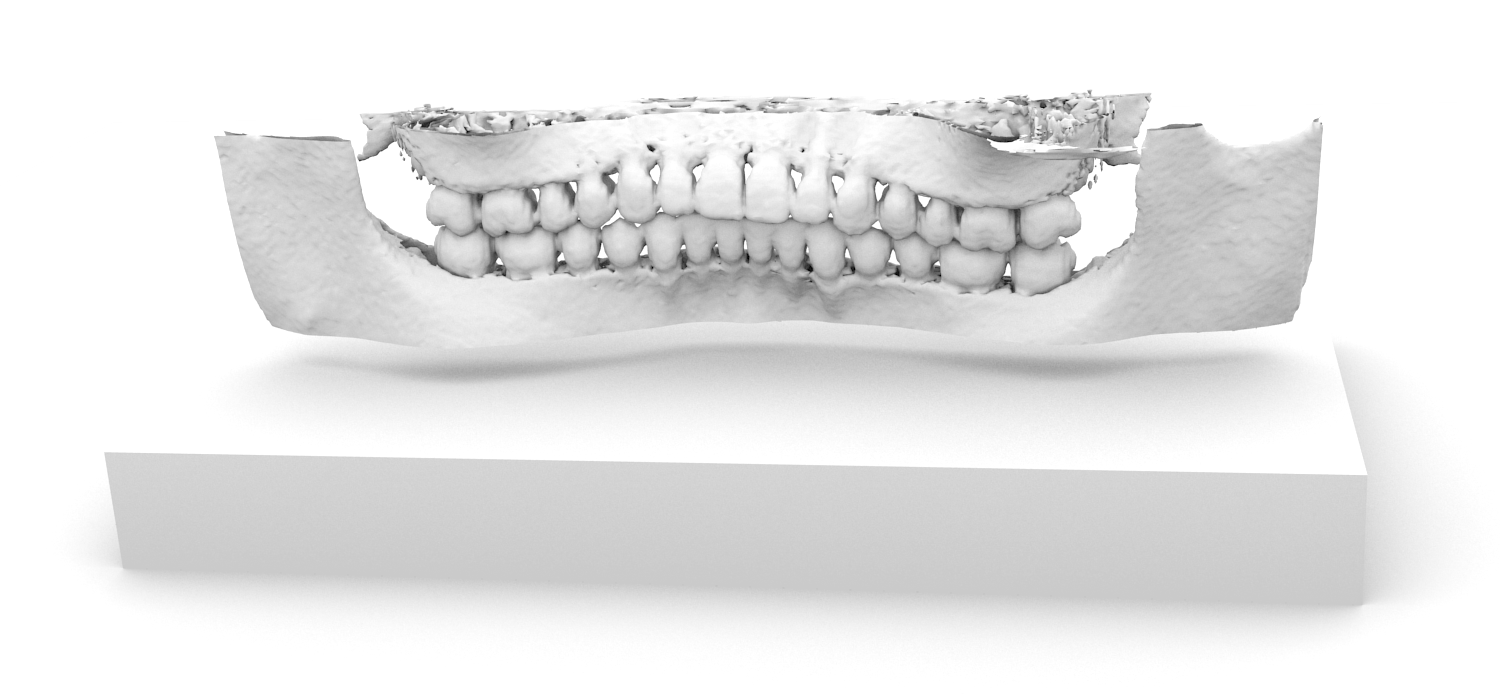
\includegraphics[width=0.8\textwidth]{Images/pano_blender.png}
\end{figure}
%
\begin{figure}
\centering
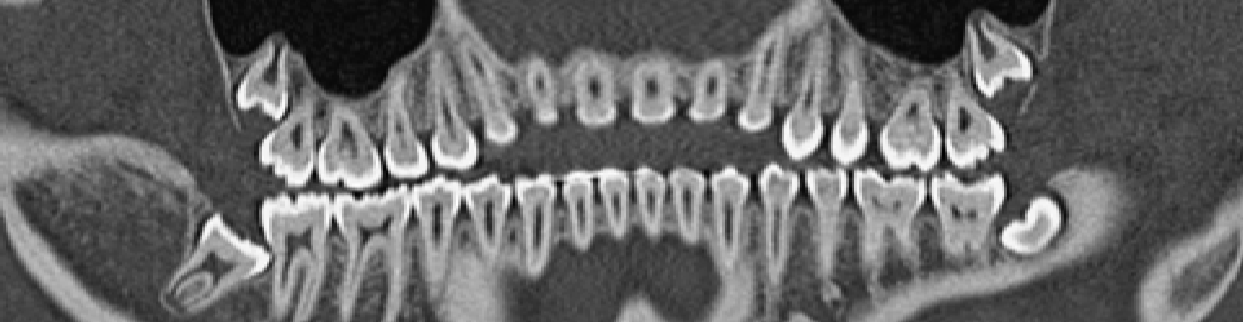
\includegraphics[width=0.8\textwidth]{Images/pano_paraview.png}
\end{figure}
%
\subsection{Straightened Curved Planar Reformation}
\cite{KAN01}

%
\section{Software Requirements}
%
\section{Conclusion}
%
%
\appendix

%%%%%%%%%%%%%%%%%%%%%%%%%%%%%%%%%%%%%%%%%
%
%  Insert the bibliography using BibTeX
%
%%%%%%%%%%%%%%%%%%%%%%%%%%%%%%%%%%%%%%%%%

\bibliographystyle{plain}
\bibliography{references}


\end{document}

